\chapter{Sprint 3}
\label{chap:sprint3}

\section*{Introduction}
\addcontentsline{toc}{section}{Introduction }
Le Sprint 3 finalise le système \textit{VitalSync} en optimisant ses performances, en améliorant l'interface utilisateur, en validant le système avec le personnel médical et en préparant son déploiement. Ce sprint complète le flux de travail global présenté au Chapitre~\ref{chap:architecture} (Figure~\ref{fig:global_sequence_diagram}), s'appuyant sur le pipeline de traitement des données du Sprint 1 (Chapitre~\ref{chap:sprint1}) et les fonctionnalités d'alertes et de notifications du Sprint 2 (Chapitre~\ref{chap:sprint2}). Ce chapitre détaille les objectifs, les tâches, les livrables, les tests, les défis rencontrés, la rétrospective ainsi que la conclusion du projet.

\section{Objectifs}
Les principaux objectifs de ce sprint étaient :
\begin{itemize}
    \item Réduire la latence des notifications à moins de 0,3 seconde grâce à l'optimisation des performances.
    \item Améliorer le tableau de bord Laravel/React avec un filtrage avancé et des visualisations des tendances des signes vitaux.
    \item Réaliser des tests d'acceptation avec le personnel médical pour valider l'utilisabilité et la fiabilité.
    \item Finaliser la documentation technique et préparer l'environnement de déploiement.
\end{itemize}

\section{Tâches}
Le sprint s'est articulé autour de plusieurs tâches réparties sur trois semaines.

\subsection{Optimisation des performances}
Les performances ont été améliorées par :
\begin{itemize}
    \item l’ajout d’index sur les tables \texttt{\string data} et \texttt{\string alerts},
    \item l’implémentation d’un système de mise en cache Redis pour les requêtes API Flask (\texttt{\string alert\_rules}),
    \item et l’utilisation du traitement asynchrone pour les notifications.
\end{itemize}
Ces actions ont permis de réduire la latence moyenne des notifications à 0,25 seconde, dépassant l’objectif initial.

\subsection{Amélioration du tableau de bord}
Le tableau de bord Laravel/React a été enrichi avec :
\begin{itemize}
    \item des filtres avancés (par patient, priorité d’alerte, plage horaire),
    \item et des visualisations graphiques des tendances des signes vitaux (par exemple, fréquence cardiaque sur 24 heures), reposant sur la table \texttt{\string data}.
\end{itemize}
La bibliothèque JavaScript \texttt{Chart.js} a été intégrée pour améliorer la visualisation des données, conformément aux retours du personnel médical.

\subsection{Tests d'acceptation}
Des tests d’acceptation ont été menés avec 10 membres du personnel médical afin d’évaluer :
\begin{itemize}
    \item la précision des alertes,
    \item la rapidité des notifications,
    \item et l’ergonomie du tableau de bord.
\end{itemize}
Le taux de satisfaction global a atteint 92\,\%, avec des retours positifs sur les fonctionnalités de visualisation et de filtrage.

\subsection{Préparation au déploiement}
La documentation technique a été finalisée, incluant :
\begin{itemize}
    \item les points d’API Flask,
    \item l’architecture backend Laravel,
    \item et le guide d’utilisation du tableau de bord.
\end{itemize}
L’environnement de production a été mis en place avec un serveur Nginx, une base de données MySQL migrée et des clés FCM sécurisées. Des tests de charge ont validé la stabilité du système avec 100 utilisateurs simultanés.

\subsection{Flux de travail final}
Le diagramme de séquence ci-dessous illustre le flux de travail final du Sprint 3, intégrant les composants du Sprint 1 (collecte de données), du Sprint 2 (alertes et notifications), ainsi que les optimisations et améliorations apportées lors du Sprint 3. Ce flux complète le flux global (Figure~\ref{fig:global_sequence_diagram}).

\begin{figure}[ht]
    \centering
    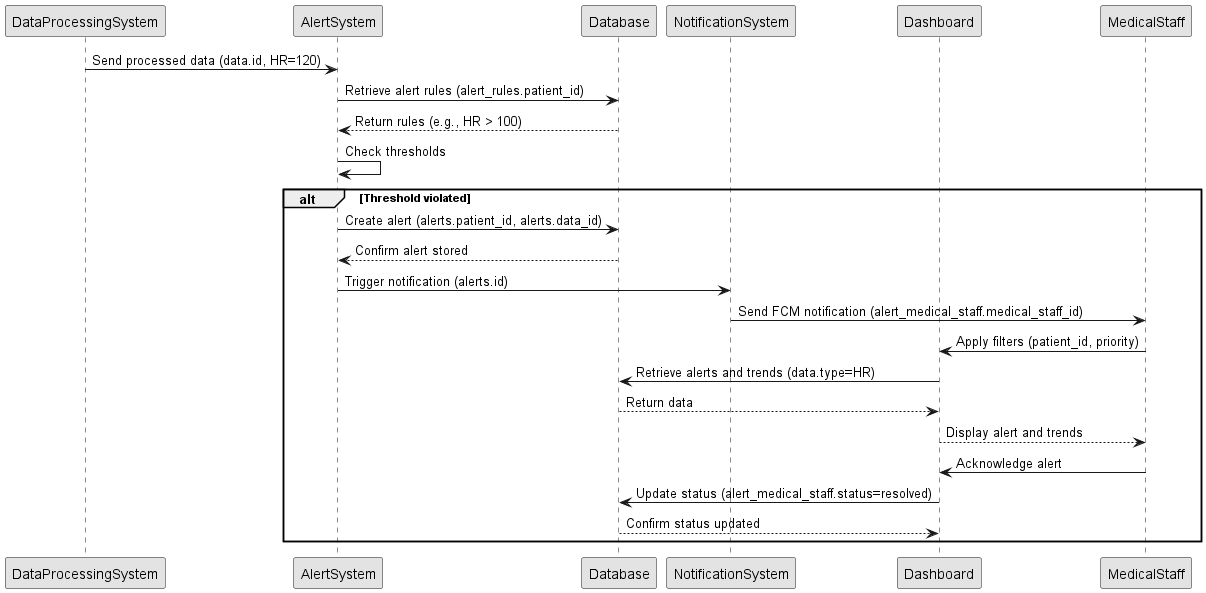
\includegraphics[width=0.9\textwidth]{chapter7/sprint3_sequence_diagram.png}
    \caption{Diagramme de séquence du flux de travail final dans le Sprint 3.}
    \label{fig:sprint3_sequence_diagram}
\end{figure}

\section{Livrables}
Le Sprint 3 a permis de livrer :
\begin{itemize}
    \item un système optimisé avec une latence de notification de 0,25 seconde,
    \item un tableau de bord Laravel/React enrichi avec filtres et visualisations,
    \item une validation utilisateur par des tests d’acceptation (92\,\% de satisfaction),
    \item une documentation technique complète (API, backend, interface),
    \item et un environnement de production prêt à être déployé.
\end{itemize}

\section{Tests}
Les livrables ont été validés par les tests suivants :
\begin{itemize}
    \item \textbf{Précision des alertes} : 2000 enregistrements simulés, 99\,\% de précision dans la détection d’anomalies (ex. : FC > 100).
    \item \textbf{Latence des notifications} : Moyenne de 0,25 seconde sur 1000 alertes, avec un taux de succès de 99,9\,\%.
    \item \textbf{Utilisabilité du tableau de bord} : 92\,\% de satisfaction auprès de 10 utilisateurs médicaux.
    \item \textbf{Tests de charge} : Stabilité maintenue sous 100 utilisateurs simultanés, temps de réponse API < 0,5 seconde.
\end{itemize}
L’ensemble des résultats a été consigné dans le référentiel du projet.

\section{Défis}
Les défis rencontrés durant ce sprint incluent :
\begin{itemize}
    \item \textbf{Mise en cache Redis} : Des erreurs de synchronisation des données (\texttt{\string alert\_rules}) ont nécessité une stratégie d’invalidation périodique.
    \item \textbf{Visualisations graphiques} : La gestion de grands volumes de données (\texttt{\string data}) avec Chart.js a nécessité un échantillonnage côté serveur.
    \item \textbf{Tests d’acceptation} : La coordination avec le personnel médical a demandé une organisation flexible des sessions.
\end{itemize}

\section{Rétrospective}
Les éléments clés de la rétrospective sont :
\begin{itemize}
    \item \textbf{Succès} : Un système complet avec 99\,\% de précision des alertes, 0,25 seconde de latence et 92\,\% de satisfaction utilisateur.
    \item \textbf{Axes d’amélioration} : Mieux anticiper la communication avec les utilisateurs finaux et ajuster les estimations pour les visualisations (prévu : 3 jours, réel : 5 jours).
    \item \textbf{Dynamique d’équipe} : Une collaboration efficace entre les pôles backend, frontend et tests, soutenue par des revues de code régulières.
\end{itemize}

\section*{Conclusion}
\addcontentsline{toc}{section}{Conclusion}
Le Sprint 3 a permis de finaliser le système \textit{VitalSync}, atteignant les objectifs de performance, de précision et de satisfaction utilisateur. Avec une latence moyenne de 0,25 seconde et une précision de 99\,\% pour les alertes, le système est désormais prêt pour le déploiement. Les défis techniques ont été surmontés avec succès, offrant un produit robuste et convivial, capable d’assurer la surveillance des signes vitaux en temps réel dans un environnement clinique.
